\documentclass[12pt, a4paper]{report}
\usepackage[utf8]{inputenc}
\usepackage[english, russian]{babel}

\usepackage{graphicx}
\usepackage{listings}
\usepackage{color}

\usepackage{amsmath}
\usepackage{pgfplots}
\usepackage{url}
\usepackage{flowchart}
\usepackage{tikz}
\DeclareGraphicsExtensions{.pdf,.png,.jpg,.svg}
\usetikzlibrary{shapes, arrows}

\usepackage{pgfplotstable}

\renewcommand\contentsname{Содержание}

\usepackage{geometry}
\geometry{left=3cm}
\geometry{right=1cm}
\geometry{top=2cm}
\geometry{bottom=2cm}

\lstset{ %
language=C++,                 % выбор языка для подсветки (здесь это С)
basicstyle=\small\sffamily, % размер и начертание шрифта для подсветки кода
numbers=left,               % где поставить нумерацию строк (слева\справа)
numberstyle=\tiny,           % размер шрифта для номеров строк
stepnumber=1,                   % размер шага между двумя номерами строк
numbersep=-5pt,                % как далеко отстоят номера строк от         подсвечиваемого кода
backgroundcolor=\color{white}, % цвет фона подсветки - используем         \usepackage{color}
showspaces=false,            % показывать или нет пробелы специальными     отступами
showstringspaces=false,      % показывать или нет пробелы в строках
showtabs=false,             % показывать или нет табуляцию в строках
frame=single,              % рисовать рамку вокруг кода
tabsize=2,                 % размер табуляции по умолчанию равен 2 пробелам
captionpos=t,              % позиция заголовка вверху [t] или внизу [b] 
breaklines=true,           % автоматически переносить строки (да\нет)
breakatwhitespace=false, % переносить строки только если есть пробел
escapeinside={\%*}{*)},   % если нужно добавить комментарии в коде
keywordstyle=\color{blue}\ttfamily,
stringstyle=\color{red}\ttfamily,
commentstyle=\color{green}\ttfamily,
morecomment=[l][\color{magenta}]{\#},
columns=fullflexible }

\usepackage{titlesec}
\titleformat{\chapter}[hang]{\LARGE\bfseries}{\thechapter{.} }{0pt}{\LARGE\bfseries}
\titleformat*{\section}{\Large\bfseries}
\titleformat*{\subsection}{\large\bfseries}

\begin{document}

    \begin{titlepage}

        \begin{center}
            \Large
            {\sl Государственное образовательное учреждение высшего профессионального образования\\
            {\bf«Московский государственный технический университет имени Н.Э. Баумана»\\
				(МГТУ им. Н.Э. Баумана)}}
				\noindent\rule{\textwidth}{2pt}
            \vspace{3cm}

			{\scshape\LARGE Лабораторная работа №1 \par}
			\vspace{0.5cm}	
			{\scshape\LARGE по курсу «Анализ алгоритмов» \par}
			\vspace{1.5cm}
			{\huge\bfseries Расстояние Левенштейна и Дамерау-Левенштейна \par}
			\vspace{2cm}
			\Large Выполнил: Сорокин А.П., гр. ИУ7-52Б\\
			\vspace{0.5cm}
			{\Large Преподаватели: Волкова Л.Л., Строганов Ю.В.}
		
			\vfill
			\Large \textit {Москва, 2019 г.}
            
        \end{center}

    \end{titlepage}
	
	\tableofcontents

	\chapter*{Введение}
	\addcontentsline{toc}{chapter}{Введение}
	
	В современном мире почти каждый человек пользуются компьютером и Интернетом в частности. Люди пишут текст в документах, выполняют поиск в поисковых системах, ищут переводы слов и текстов в онлайн-словарях. В таких ситуациях человек часто делает орфографические ошибки или опечатки, и на их исправление он тратит своё время. Чтобы этого избежать, в подобных системах есть опции поиска ошибок и автоисправления. Для такой опции необходим поиск расстояния между строками по алгоритмам Левенштейна и Дамерау-Левенштейна. Также эта задача необходима и в программировании (например, для сравнения текстовых файлов или файлов кода в системах контроля версий) и в биоинформатике (например, для сравнения белков, генов и хромосом).

    \chapter{Аналитическая часть}

	\section{Задачи}
	Цель лабораторной работы: исследовать расстояния Левенштейна и Дамерау-Левенштейна. Для достижения этой цели были поставлены следующие задачи: 
	\begin{itemize}
		\item изучить алгоритмы вычисления расстояний между строками;
		\item применить метод динамического программирования для матричных реализаций алгоритмов;
		\item сравнить матричную и рекурсивную реализации алгоритмов;
		\item оценить эффективность каждой из реализаций по времени и памяти.
	\end{itemize}

	\section{Описание алгоритмов}
	\subsection{Расстояние Левенштейна}
	Расстояние Левенштейна определяет минимальное количество операций, необходимых для превращения одной строки в другую, среди которых:
	\begin{itemize}
		\item вставка (I - insert);
		\item удаление (D - delete);
		\item замена (R - replace).
	\end{itemize}
	У каждой операции есть так называемая "цена", или "штраф" за её выполнение. Цена каждой операции равна 1, кроме случая совпадения символов (M - match); цена в этом случае равна 0, т. к. при равенстве символов не требуется никаких действий. Соответственно, задача нахождения расстояния Левенштейна заключается в нахождении такой последовательности операции, приводящик одну строку к другой, суммарная цена которых минимальна.

	Таким образом, если заданы две строки $S_{1}$ и $S_{2}$ с длинами $m$ и $n$ соответственно над некоторым алфавитом, то расстояние Левенштейна $D(S_{1}, S_{2})$ между данными строками можно вычислить по следующей рекуррентной формуле \cite{recurs}:

	\begin{equation}
	\label{formula_leven}
	D(S_{1}[1..m], S_{2}[1..n]) =
		\begin{cases}
		m\ if\ n = 0\\
		n\ if\ m = 0\\
		min \begin{cases}
		D(S_{1}[1..m-1], S_{2}[1..n] + 1)\\
		D(S_{1}[1..m], S_{2}[1..n-1]+1)\\
		D(S_{1}[1..m-1], S_{2}[1..n-1]+(S_{1}[m] \neq S_{2}[n]))
		\end{cases}
	\end{cases}
	\end{equation}
	
	Соотношения в рекурретной формуле отвечают за соотвествующие разрешённые операции:
	\begin{enumerate}
		\item Вставка.
		\item Удаление.
		\item Замена или совпадение в зависимости от результата $(S_{1}[m] \neq S_{2}[n])$.	
	\end{enumerate}

	\subsection{Расстояние Дамерау-Левенштейна}
	Расстояние Дамерау-Левенштейна является модификацией расстояние Левенштейна. К исходному набору возможных операций добавляется операция транспозиции (T - transpose), или перестановка двух соседних символов. В своих исследованиях Ф. Дамерау показал, что наиболее частой ошибкой при вводе текста является перестановка двух соседних букв слов ~\cite{damerau}. "Цена" данной операции также равняется 1. При вычислении расстояния Левенштейна в такой ситуации потребовалось бы дважды заменить символ. Суммарная цена этих двух операций равнялась бы 2, а транспозиция добавляет в суммарную цену лишь 1. Исходя из этого, можно утверждать, что расстояние Дамерау-Левенштейна даёт лучший результат в сравнении с расстоянием Левенштейна.
	
	При вычислении расстояния Дамерау-Левенштейна в рекурретную формулу вносится дополнительное соотношение в минимум:
	\begin{equation}
	\label{damerau_eq}
	D(S_{1}[1..m-2], S_{2}[1..n-2])+1
	\end{equation}
	Соотношение ~(\ref{damerau_eq}) вносится в выражение только при выполнении следующих условий:
	\begin{equation}
	\label{damerau_conditions}
	\begin{cases}
		m > 2,n > 2\\
		S_{1}[m] = S_{2}[n-1]\\
		S_{1}[m-1] = S_{2}[n]
	\end{cases}	
	\end{equation}
	
	Таким образом получаем следующую рекурретную формулу:
	
	\begin{equation}
	\label{formula_damerau}
	D(S_{1}[1..m],S_{2}[1..n]) = \begin{cases}
	m\ if\ n = 0\\
	n\ if\ m = 0\\
	min \begin{cases}
		D(S_{1}[1..m-1], S_{2}[1..n] + 1)\\
		D(S_{1}[1..m], S_{2}[1..n-1]+1)\\
		D(S_{1}[1..m-1], S_{2}[1..n-1]+(S_{1}[m] \neq S_{2}[n]))\\
		D(S_{1}[1..m-2], S_{2}[1..n-2])+1
	\end{cases} & \mbox{if ~(\ref{damerau_conditions})}\\	
	min \begin{cases}
		D(S_{1}[1..m-1], S_{2}[1..n] + 1)\\
		D(S_{1}[1..m], S_{2}[1..n-1]+1)\\
		D(S_{1}[1..m-1], S_{2}[1..n-1]+(S_{1}[m] \neq S_{2}[n]))
	\end{cases} & \mbox{otherwise}\\
	\end{cases}
	\end{equation}

	\chapter{Конструкторская часть}
	
	\section{Схемы алгоритмов}
	На рисунках 2.1 - 2.3 представлены схемы алгоритмов трёх реализаций алгоритмов поиск расстояния между строками.
	\begin{figure}[ht!]
		\centering
		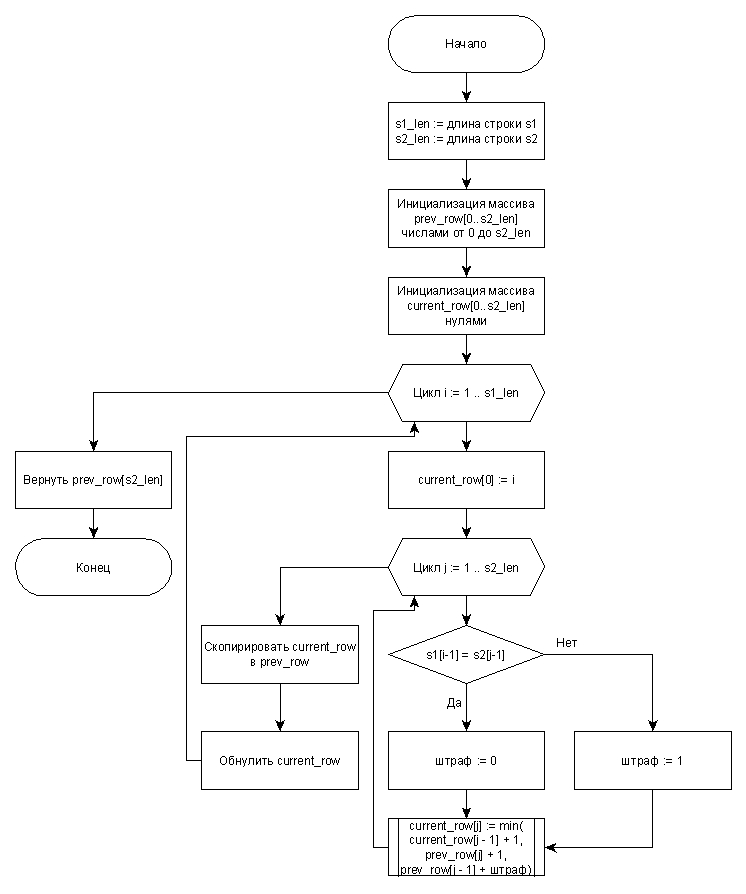
\includegraphics[scale=0.5]{leven}
		\caption{Матричная реализация алгоритма Левенштейна}
		\label{fig:leven}
	\end{figure}

	\begin{figure}[ht!]
		\centering
		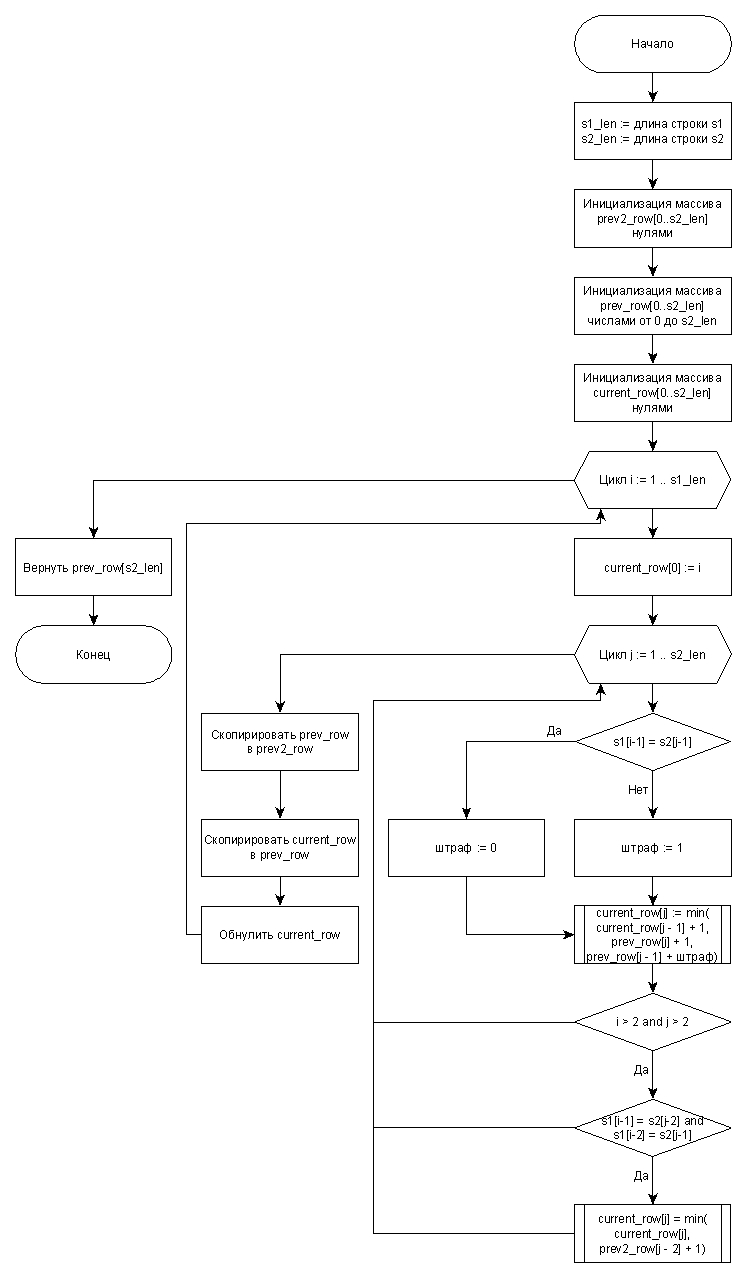
\includegraphics[scale=0.5]{damleven}
		\caption{Матричная реализация алгоритма Дамерау-Левенштейна}
		\label{fig:damleven}
	\end{figure}

	\begin{figure}
		\centering
		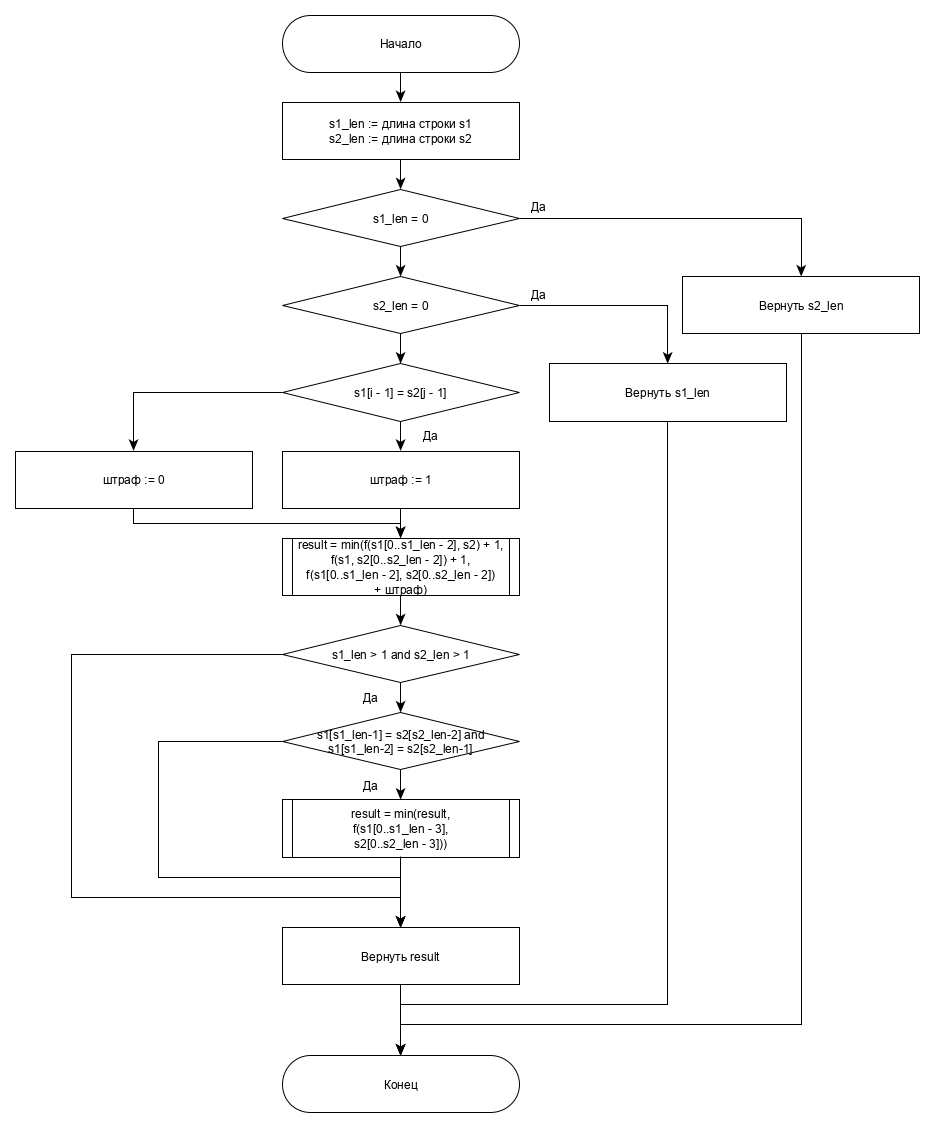
\includegraphics[scale=0.5]{damleven_r}
		\caption{Рекурсивная реализация алгоритма Дамерау-Левенштейна}
		\label{fig:damlevenr}
	\end{figure}

	\newpage
	
	\chapter{Технологическая часть}
	\section{Требования к программному обеспечению}
	На вход подаются две строки максимальной длины в 50 символов, которые входят в таблицу Юникода (UTF-8). На выход программа выдаёт три числовых значения, которые являются результатами вычисления расстояний тремя методам: матричными реализациями алгоритмов Левенштейна и Дамерау-Левенштейна и рекурсивной реализацией алгоритма Дамерау-Левенштейна. В качестве результата для матричных реализаций также выводится матрица расстояний.
	\section{Средства реализации}
	Для реализации программы был использован язык C++ ~\cite{CPP}. Для замера процессорного времени была использована функция rdtsc() из библиотеки stdrin.h.
	\section{Реализации алгоритмов}
	На листингах 3.1 - 3.3 представлены коды реализации алгоритмов поиска расстояния.
	\begin{lstlisting}[label=some-code,caption=Матричная реализация алгоритма Левенштейна]
	unsigned levenshtein(std::string s1, std::string s2, bool to_print)
	{
		size_t s1_len = s1.length(), s2_len = s2.length();
		size_t row_length = s2_len + 1;
		unsigned row_bytes = row_length * sizeof(unsigned);
		
		unsigned *prev_row = new unsigned[row_length];
		unsigned *current_row = new unsigned[row_length];
		for (size_t i = 0; i < row_length; i++)
		prev_row[i] = i;
		
		if (to_print)
		{
			for (size_t i = 0; i < row_length; i++)
				std::cout << prev_row[i] << ' ';
			std::cout << std::endl;
		}
		
		for (size_t i = 1; i <= s1_len; i++)
		{
			current_row[0] = i;
			for (size_t j = 0; j < row_length; j++)
			{
				unsigned match_fault = unsigned(s1[i - 1] != s2[j - 1]);
				current_row[j] = std::min({current_row[j - 1] + 1,
											prev_row[j] + 1,
											prev_row[j - 1] + match_fault});
			}
			if (to_print)
			{
				for (size_t k = 0; k < row_length; k++)
					std::cout << current_row[k] << ' ';
				std::cout << std::endl;
			}
			memcpy(prev_row, current_row, row_bytes);
		}
		
		unsigned result = current_row[s2_len];
		
		delete [] prev_row;
		delete [] current_row;
		
		return result;
	}
	\end{lstlisting}

	\begin{lstlisting}[label=some-code,caption=Матричная реализация алгоритма Дамерау-Левенштейна]
	unsigned damerau(std::string s1, std::string s2, bool to_print)
	{
		size_t s1_len = s1.length(), s2_len = s2.length();
		size_t row_length = s2_len + 1;
		unsigned row_bytes = row_length * sizeof(unsigned);
		
		unsigned *prev2_row = new unsigned[row_length];
		unsigned *prev_row = new unsigned[row_length];
		unsigned *current_row = new unsigned[row_length];
		for (size_t i = 0; i < row_length; i++)
		{
			prev2_row[i] = 0;
			prev_row[i] = i;
		}
		
		if (to_print)
		{
			for (size_t i = 0; i < row_length; i++)
				std::cout << prev_row[i] << ' ';
			std::cout << std::endl;
		}
		
		for (size_t i = 1; i <= s1_len; i++)
		{
			current_row[0] = i;
			for (size_t j = 0; j < row_length; j++)
			{
				unsigned match_fault = unsigned(s1[i - 1] != s2[j - 1]);
				current_row[j] = std::min({current_row[j - 1] + 1,
											prev_row[j] + 1,
											prev_row[j - 1] + match_fault});
				if (i >= 2 && j >= 1)
					if (s1[i - 1] == s2[j - 2] && s1[i - 2] == s2[j - 1])
						current_row[j] = std::min(current_row[j],
													prev2_row[j - 2] + 1);
			}
		
			if (to_print)
			{
				for (size_t k = 0; k < row_length; k++)
					std::cout << current_row[k] << ' ';
				std::cout << std::endl;
			}
		
			memcpy(prev2_row, prev_row, row_bytes);
			memcpy(prev_row, current_row, row_bytes);
		}
	
		unsigned result = current_row[s2_len];
	
		delete [] prev2_row;
		delete [] prev_row;
		delete [] current_row;
	
		return result;
	}
	\end{lstlisting}

	\begin{lstlisting}[label=some-code,caption=Рекурсивная реализация алгоритма Дамерау-Левенштейна]
	unsigned damerau_r(std::string s1, std::string s2, bool to_print)
	{
		size_t s1_len = s1.length(), s2_len = s2.length();
		if (s1_len == 0)
			return s2_len;
		if (s2_len == 0)
			return s1_len;
		
		unsigned match_fault = unsigned(s1[s1_len - 1] != s2[s2_len - 1]);
		
		unsigned result = std::min({damerau_r(s1.substr(0, s1_len - 1),
									s2.substr(0, s2_len)) + 1,
									damerau_r(s1.substr(0, s1_len),
									s2.substr(0, s2_len - 1)) + 1,
									damerau_r(s1.substr(0, s1_len - 1),
									s2.substr(0, s2_len - 1)) + match_fault});
		
		if (s1_len > 1 && s2_len > 1)
			if (s1[s1_len - 1] == s2[s2_len - 2] &&
				s1[s1_len - 2] == s2[s2_len - 1])
				return std::min(result, damerau_r(s1.substr(0, s1_len - 2),
													s2.substr(0, s2_len - 2)) + 1);
		
		return result;
	}
	\end{lstlisting}

	\newpage

	\section{Тесты}
	Для проверки корректности работы были подготовлены функциональные тесты, представленные в таблице 3.1. В данной таблице $\lambda$ означает пустую строку, а числа в столбцах "Ожидание" и "Результат" соответствуют результатам работы алгоритмов в следующем порядке:
	\begin{enumerate}
		\item Матричная реализация алгоритма Левенштейна.
		\item Матричная реализация алгоритма Дамерау-Левенштейна.
		\item Рекурсивная реализация алгоритма Дамерау-Левенштейна.
	\end{enumerate}

	\begin{table}[ht!]
		\caption{Функциональные тесты}
		\begin{center}
			\begin{tabular}{|c|c|c|c|}
			\hline
			\bf{Строка 1} & \bf{Строка 2} & \bf{Ожидание} & \bf{Результат}\\\hline
			$\lambda$ & $\lambda$ & 0 0 0 & 0 0 0\\\hline
			$\lambda$ & а & 1 1 1 & 1 1 1\\\hline
			а & $\lambda$ & 1 1 1 & 1 1 1\\\hline
			а & а & 0 0 0 & 0 0 0\\\hline
			а & б & 1 1 1 & 1 1 1\\\hline
			азы & базы & 1 1 1 & 1 1 1\\\hline
			компютер & компьютер & 1 1 1 & 1 1 1\\\hline
			данны & данные & 1 1 1 & 1 1 1\\\hline
			email.ru & mail.ru & 1 1 1 & 1 1 1\\\hline
			programmmer & programmer & 1 1 1 & 1 1 1\\\hline
			mail.rus & mail.ru & 1 1 1 & 1 1 1\\\hline
			ашибка & ошибка & 1 1 1 & 1 1 1\\\hline
			алгоритм & алгорифм & 1 1 1 & 1 1 1\\\hline
			копия & копии & 1 1 1 & 1 1 1\\\hline
			укрсовой & курсовой & 2 1 1 & 2 1 1\\\hline
			аглоритм & алгоритм & 2 1 1 & 2 1 1\\\hline
			унивре & универ & 2 1 1 & 2 1 1\\\hline
			курс & курсовой & 4 4 4 & 4 4 4\\\hline
			курсовой & курс & 4 4 4 & 4 4 4\\\hline
			курсовой & курсовик & 2 2 2 & 2 2 2\\\hline
			код & закодировать & 9 9 9 & 9 9 9\\\hline
			закодировать & код & 9 9 9 & 9 9 9\\\hline
			ccoders & recoding & 5 5 5 & 5 5 5\\\hline
			header & subheader & 3 3 3 & 3 3 3\\\hline
			subheader & header & 3 3 3 & 3 3 3\\\hline
			subheader & overheader & 4 4 4 & 4 4 4\\\hline
			\end{tabular}
		\end{center}
	\end{table}

	В результате проверки все реализации алгоритмов прошли все поставленные функциональные тесты.

	\chapter{Экспериментальная часть}
	\section{Примеры работы}
	На рисунке 4.1 представлен пример работы программы, демонстрирующий различие в работе алгоритмов наглядно: различаются матрицы расстояний и результаты.
	\begin{figure}[ht!]
		\centering
		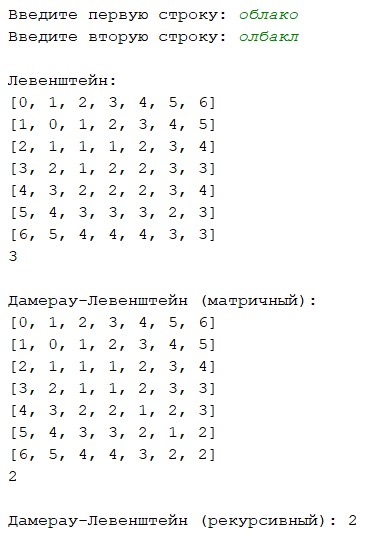
\includegraphics[width=0.5\linewidth]{example.jpg}
		\caption{Пример работы программы}
		\label{fig:example}
	\end{figure}
	
	\section{Сравнение работы алгоритмов Левенштейна и Дамерау-Левенштейна}
	Для сравнения времени работы алгоритмов Левенштейна и Дамерау-Левенштейна были использованы строки длиной от 10 до 70 с шагом 10. Эксперимент для более точного результата повторялся 100 раз. Итоговый результат рассчитывался как средний из полученных результатов. Результаты измерений показаны в таблице 4.1 и на рисунке 4.2.\\
	\begin{table}[ht!]
		\caption{Время работы матричных реализаций алгоритмов в тактах процессора}
		\begin{center}
			\pgfplotstabletypeset[
			col sep=semicolon,
			string type,
			columns/Size/.style={column name=Длина слова, column type={|c}},
			columns/Leven/.style={column name=Алгоритм Левенштейна, column type={|c}},
			columns/Damerau/.style={column name=Алгоритм Дамерау-Левенштейна, column type={|c|}},
			every head row/.style={before row=\hline,after row=\hline},
			every last row/.style={after row=\hline},
			]{MatrixTime.csv}
		\end{center}
	\end{table}
	
	\begin{figure}[ht!]
		\begin{tikzpicture}
		\begin{axis}
			[%title = График времени работы матричных реализаций алгоритмов Левенштейна и Дамерау-Левенштейна,
			table/col sep = semicolon,
			xlabel={Количество символов},
			ylabel={Время в тиках},
			ymin = 0,
			legend pos=outer north east,
			ymajorgrids=true,
			grid style=dashed]
			\addplot[color=red, mark=*] table[x={Size}, y={Leven}] {MatrixTime.csv};
			\addplot[color=blue, mark=*] table[x={Size}, y={Damerau}] {MatrixTime.csv};
			\legend{Алгоритм Левенштейна, Алгоритм Дамерау-Левенштейна}
		\end{axis}
		\end{tikzpicture}
		\caption{График времени работы матричных реализаций алгоритмов Левенштейна и Дамерау-Левенштейна}
	\end{figure}
	
	Алгоритм Левенштейна выигрывает по времени в среднем не более, чем на 10\%. Алгоритм Дамерау-Левенштейна выполняется дольше за счёт добавления небольшого количества операций.
   
	\section{Сравнение работы реализаций алгоритма Дамерау-Левенштейна}
	Для сравнения времени работы матричной и рекурсивной реализаций алгоритма Дамерау-Левенштейна были использованы строки длиной от 1 до 10 с шагом 1. Эксперимент для более точного результата повторялся 100 раз. Итоговый результат рассчитывался как средний из полученных результатов. Результаты измерений показаны в таблице 4.2 и на рисунках 4.3 и 4.4.\\
	
	\begin{table}[ht!]
		\begin{center}
			\caption{Время работы реализаций алгоритма Дамерау-Левенштейна в тактах процессора}
			\pgfplotstabletypeset[
			col sep=semicolon,
			string type,
			columns/Size/.style={column name=Длина слова, column type={|c}},
			columns/Matrix/.style={column name=Матричная реализация, column type={|c}},
			columns/Recursive/.style={column name=Рекурсивная реализация, column type={|c|}},
			every head row/.style={before row=\hline,after row=\hline},
			every last row/.style={after row=\hline},
			]{DamerauTime.csv}
		\end{center}
	\end{table}

	\begin{figure}[ht!]
		\begin{tikzpicture}
			\begin{axis}
			[%title = График времени работы матричной реализации алгоритма Дамерау-Левенштейна,
			table/col sep = semicolon,
			xlabel={Количество символов},
			ylabel={Время в тиках},
			ymin = 0,
			legend pos=outer north east,
			ymajorgrids=true,
			grid style=dashed]
			\addplot[color=red, mark=*] table[x={Size}, y={Matrix}] {DamerauTime.csv};
			\end{axis}
		\end{tikzpicture}
		\caption{График времени работы матричной реализации алгоритма Дамерау-Левенштейна}
	\end{figure}
	
	\begin{figure}[ht!]
		\begin{tikzpicture}
			\begin{axis}
			[%title = График времени работы рекурсивной реализации алгоритма Дамерау-Левенштейна,
			table/col sep = semicolon,
			xlabel={Количество символов},
			ylabel={Время в тиках},
			ymin = 0,
			legend pos=outer north east,
			ymajorgrids=true,
			grid style=dashed]
			\addplot[color=blue, mark=*] table[x={Size}, y={Recursive}] {DamerauTime.csv};
			\end{axis}
		\end{tikzpicture}
		\caption{График времени работы рекурсивной реализации алгоритма Дамерау-Левенштейна}
	\end{figure}
	
 	Время выполнения рекурсивной реализации алгоритма резко возрастает с увеличением длины слов: так при длине слова 5 рекурсивная выполняется в 15 раз дольше, чем матричная, а при длине слова 10 - приблизительно в 40000 раз. Рекурсивная реализация выигрывает по времени только при длине слов, равной 1 (в 2 раза), но это тривиальный случай. Можно сделать вывод о том, что матричная реализация алгоритма значительно эффективнее рекурсивной при любой длине слова.

	\chapter*{Заключение}
	\addcontentsline{toc}{chapter}{Заключение}
	В ходе лабораторной работы были изучены и реализованы алгоритмы нахождения расстояния Левенштейна и Дамерау-Левенштейна. Для этого были реализованы три различные реализации алгоритмов с применением навыка динамического программирования для матричных.\\
	Экспериментально потверждена эффективность матричных реализаций над рекурсивной: при длине слов выше 10 символов применение рекурсивной реализации алгоритма Дамерау-Левенштейна является нецелесообразной, т. к. проигрывает по памяти и по времени матричных в несколько порядков. Также было экспериментально установлено, что применение матричной реализации Дамерау-Левенштейна допустимо, так как данный алгоритм уступает по времени алгоритму Левенштейна лишь на 10\%, но при это при решении определённых задач может давать меньший результат.
	\newpage
	
	\begin{thebibliography}{}
	\bibitem{leven} Двоичные коды с исправлением выпадений, вставок и замещений символов. Доклады Академий Наук СССР, 1965. В. И. Левенштейн.
	\bibitem{damerau} A technique for computer detection and correction of spelling errors. Damerau Fred J.
	\bibitem{recurs} Indexing methods for approximate dictionary searching. Journal of Experimental Algorithmics, 2011. L. M. Boytsov
	\bibitem{CPP} https://cppreference.com/ [Электронный ресурс]
	\end{thebibliography}
	\addcontentsline{toc}{chapter}{Литература}

\end{document}
